\documentclass[11pt]{article}
\usepackage[a4paper,margin=1in]{geometry}
\usepackage{amsmath,amssymb,mathtools}
\usepackage{siunitx}
\usepackage{enumitem}
\usepackage{booktabs}
\usepackage{physics}
\usepackage{bm}
\usepackage{microtype}
\usepackage{titlesec}
\usepackage{tikz}
\usepackage{pgfplots}
\usepackage{subcaption}
\usepackage{float}
\pgfplotsset{compat=1.18}
\titleformat{\section}{\large\bfseries}{}{0em}{}[\titlerule]
\titleformat{\subsection}{\normalsize\bfseries}{}{0em}{}
\setlength{\parskip}{0.35em}
\setlength{\parindent}{0pt}

\title{EE 115 — Homework 1: Solutions}
\author{Kaushik Vada}
\date{\today}

\begin{document}
 \maketitle
\begin{center}
\emph{Fourier series/transform, complex envelopes, DSB--SC demod}
\end{center}
\vspace{0.5em}

\section*{Problem 1}
A real, periodic signal $m(t)=m(t+T)$ is defined over one symmetric period ($|t|<T/2$) by
\[
m(t)=
\begin{cases}
-3, & -\tfrac{T}{3}\le t<0,\\[2pt]
\phantom{-}3, & 0\le t<\tfrac{T}{3},\\[2pt]
0, & \text{otherwise on }(-\tfrac{T}{2},\tfrac{T}{2}),
\end{cases}
\]
and extended periodically.

\subsection*{(a) Mean, energy in $|t|<T/2$, and average power}
\textbf{Mean.} Over any period, areas cancel by odd symmetry:
\[
\bar m=\frac{1}{T}\!\int_{-T/2}^{T/2}\! m(t)\,dt
= \frac{1}{T}\Big[3\cdot\tfrac{T}{3}+(-3)\cdot\tfrac{T}{3}\Big]=0.
\]

\textbf{Energy within $|t|<T/2$.} On $(-T/2,T/2)$ the signal is $\pm3$ on a total length $2(T/3)$ and $0$ elsewhere, so
\[
E_{|t|<T/2}=\int_{-T/2}^{T/2} m^2(t)\,dt
= 9\cdot\frac{2T}{3}=6T.
\]

\textbf{Average power.} For a periodic signal, $P_{\text{avg}}=\dfrac{1}{T}\int_{-T/2}^{T/2} m^2(t)\,dt= \dfrac{6T}{T}=6.$

\subsection*{(b) Exponential Fourier series coefficients}
Let $\omega_0=\tfrac{2\pi}{T}$ and $k\in\mathbb{Z}$. With
\[
c_k=\frac{1}{T}\int_{-T/2}^{T/2} m(t)\,e^{-j k\omega_0 t}\,dt,
\]
only the two nonzero subintervals contribute:
\begin{align*}
c_k
&=\frac{1}{T}\!\left(\int_{0}^{T/3} 3\,e^{-j k\omega_0 t}\,dt
+\int_{-T/3}^{0} (-3)\,e^{-j k\omega_0 t}\,dt\right)\\
&=\frac{3}{T}\left[\frac{e^{-jk\omega_0 t}}{-j k\omega_0}\right]_{0}^{T/3}
-\frac{3}{T}\left[\frac{e^{-jk\omega_0 t}}{-j k\omega_0}\right]_{-T/3}^{0}\\
&=\frac{3}{-j k\omega_0 T}\Big(e^{-j\frac{2\pi k}{3}}-1\Big)
+\frac{3}{j k\omega_0 T}\Big(1-e^{\,j\frac{2\pi k}{3}}\Big)\\
&=\frac{6}{j k\omega_0 T}\Big(1-\cos\tfrac{2\pi k}{3}\Big)
= -\,j\,\frac{6}{2\pi k}\Big(1-\cos\tfrac{2\pi k}{3}\Big).
\end{align*}
Thus for $k\neq 0$,
\[
\boxed{\; c_k = -\,j\,\frac{3}{\pi k}\Big(1-\cos\tfrac{2\pi k}{3}\Big)
= -\,j\,\frac{6}{\pi k}\,\sin^2\!\Big(\frac{\pi k}{3}\Big)\;}
\]
and since $m(t)$ is odd and real, $\boxed{c_0=0}$, each $c_k$ is \emph{purely imaginary} (no cosine terms), and $c_{-k}=-c_k$ (odd in $k$).\\
A convenient simplification uses the $3$-periodicity of $\cos(2\pi k/3)$:
\[
\cos\!\Big(\tfrac{2\pi k}{3}\Big)=
\begin{cases}
1, & 3\,|\,k,\\[2pt]
-1/2, & 3\nmid k,
\end{cases}
\qquad\Rightarrow\qquad
\boxed{\;c_k=
\begin{cases}
0, & 3\,|\,k,\\[2pt]
-\,j\,\dfrac{9}{2\pi k}, & 3\nmid k~.
\end{cases}}
\]

\subsection*{(c) Real and imaginary parts of $M(f)$ for $|f|<\tfrac{6}{T}$}
For a periodic signal, the Fourier transform is a line spectrum:
\[
M(f)=\sum_{k=-\infty}^{\infty} c_k\,\delta\!\left(f-\frac{k}{T}\right).
\]
Here $c_k$ are purely imaginary and vanish for $k$ divisible by $3$. Therefore
\[
\Re\,M(f)\equiv 0,\qquad
\Im\,M(f)=\sum_{k\in\mathbb{Z}\setminus\{0\}}\Im\{c_k\}\,\delta\!\left(f-\frac{k}{T}\right),
\]
with $\Im\{c_k\}=-\frac{9}{2\pi k}$ for $k\equiv\pm1,\pm2\pmod 3$, and $0$ for $k\equiv 0\pmod 3$.
The first few impulses (``sketch data'') within $\abs{f}<6/T$:
\[
\begin{array}{c|ccccccccccc}
k & -5 & -4 & -3 & -2 & -1 & 0 & 1 & 2 & 3 & 4 & 5\\\hline
f=\tfrac{k}{T} & -\tfrac{5}{T}&-\tfrac{4}{T}&-\tfrac{3}{T}&-\tfrac{2}{T}&-\tfrac{1}{T}&0&
\tfrac{1}{T}&\tfrac{2}{T}&\tfrac{3}{T}&\tfrac{4}{T}&\tfrac{5}{T}\\
\Im\{c_k\} & \tfrac{9}{10\pi} & \tfrac{9}{8\pi} & 0 & \tfrac{9}{4\pi} & \tfrac{9}{2\pi} & 0 &
-\tfrac{9}{2\pi} & -\tfrac{9}{4\pi} & 0 & -\tfrac{9}{8\pi} & -\tfrac{9}{10\pi}
\end{array}
\]
(Real part is identically zero.)

\begin{figure}[H]
\centering
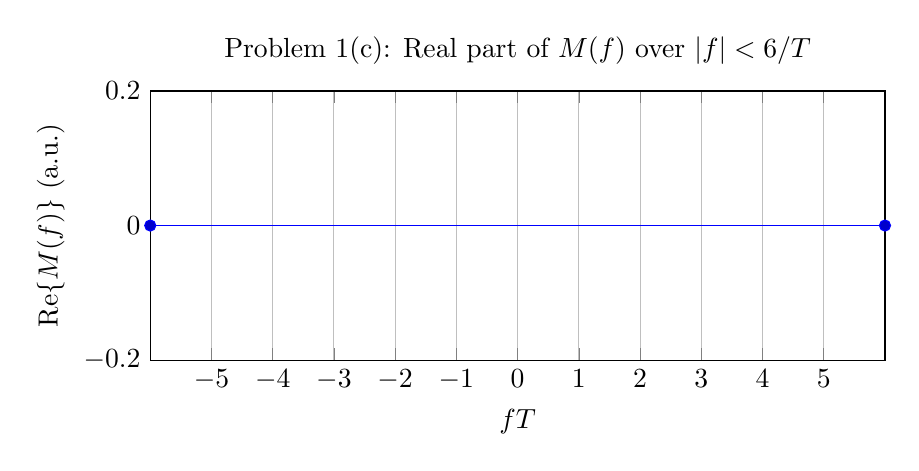
\begin{tikzpicture}
\begin{axis}[
    width=0.9\linewidth,
    height=5cm,
    xlabel={$fT$},
    ylabel={$\Re\{M(f)\}$ (a.u.)},
    ymin=-0.2, ymax=0.2,
    xmin=-6, xmax=6,
    xtick={-5,-4,-3,-2,-1,0,1,2,3,4,5},
    ytick={-0.2,0,0.2},
    grid=both,
    title={Problem 1(c): Real part of $M(f)$ over $|f|<6/T$}
]
% Real part is identically zero
\addplot+[domain=-6:6, samples=2] {0};
\end{axis}
\end{tikzpicture}
\caption{Real part $\Re\{M(f)\}$ is identically zero because $m(t)$ is odd.}
\end{figure}

\begin{figure}[H]
\centering
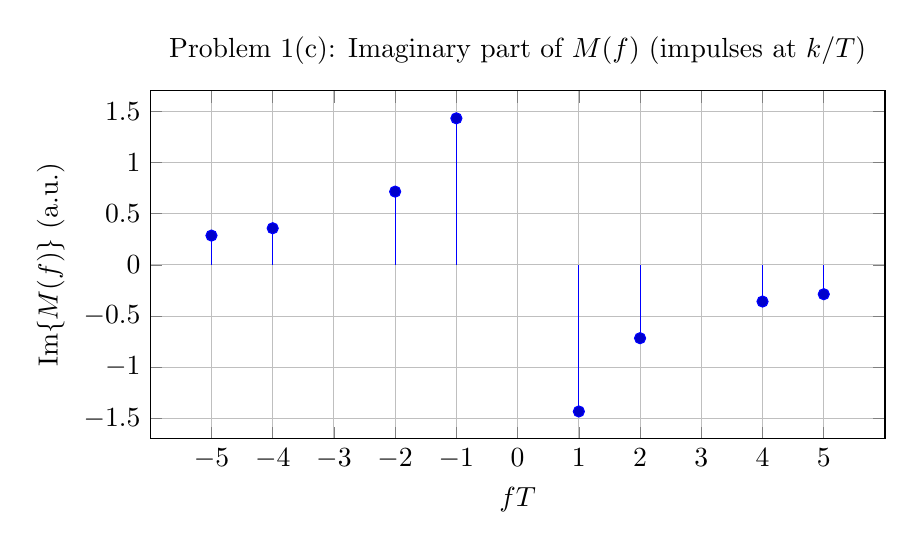
\begin{tikzpicture}
\begin{axis}[
    width=0.9\linewidth,
    height=6cm,
    xlabel={$fT$},
    ylabel={$\Im\{M(f)\}$ (a.u.)},
    xmin=-6, xmax=6,
    ymin=-1.7, ymax=1.7,
    xtick={-5,-4,-3,-2,-1,0,1,2,3,4,5},
    ytick={-1.5,-1.0,-0.5,0,0.5,1.0,1.5},
    grid=both,
    title={Problem 1(c): Imaginary part of $M(f)$ (impulses at $k/T$)}
]
% Impulses: Imag{c_k} = -9/(2\pi k) for k = \pm1,\pm2,\pm4,\pm5; zero for k=0,\pm3
\addplot+[ycomb, mark=*] coordinates
{(-5, 0.28648) (-4, 0.35810) (-2, 0.71620) (-1, 1.43239) (1, -1.43239) (2, -0.71620) (4, -0.35810) (5, -0.28648)};
\end{axis}
\end{tikzpicture}
\caption{Imaginary part $\Im\{M(f)\}$ showing nonzero spectral lines at $k/T$ for $k\equiv \pm1,\pm2\ (\mathrm{mod}\ 3)$. Values use $\Im\{c_k\}=-9/(2\pi k)$.}
\end{figure}

\section*{Problem 2}
For a real passband $x(t)$, the complex envelope $g(t)$ \emph{with respect to} $\cos(2\pi f_c t)$ is the baseband signal satisfying
\[
x(t)=\Re\{\,g(t)\,e^{j2\pi f_c t}\,\}.
\]

\subsection*{(a) $x(t)=a(t)\cos(2\pi f_c t+\theta(t))+b(t)\cos(2\pi f_c t+\phi(t))$}
Each cosine term has envelope equal to its complex phasor:
\[
\boxed{\;g(t)=a(t)\,e^{j\theta(t)}+b(t)\,e^{j\phi(t)}\;}
\]
since $\Re\{a e^{j\theta}e^{j2\pi f_c t}\}=a\cos(2\pi f_c t+\theta)$ (and similarly for the $b$ term).

\subsection*{(b) $x(t)=a(t)\cos(2\pi f_c t)-b(t)\sin(2\pi f_c t)+c(t)\sin(2\pi f_c t+\phi(t))$}
Use the standard $I/Q$ identity $\Re\{(I+jQ)e^{j\omega_c t}\}=I\cos\omega_c t - Q\sin\omega_c t$ and
$\sin(\omega_c t+\phi)=\sin\omega_c t\cos\phi+\cos\omega_c t\sin\phi$. Grouping coefficients:
\[
I(t)=a(t)+c(t)\sin\phi(t),\qquad Q(t)=b(t)-c(t)\cos\phi(t),
\]
so
\[
\boxed{\;g(t)=I(t)+jQ(t)=a(t)+j\,b(t)+c(t)\,e^{\,j(\phi(t)-\frac{\pi}{2})}\;}
\]
(\,equivalently $a+j b + c\sin\phi + j\,[\,b-c\cos\phi\,]$\,).

\subsection*{(c) $x(t)=a(t)\sin\!\big(2\pi(f_c+\Delta)t+\theta(t)\big)$}
Write $\sin(\cdot)=\Re\{e^{j(\cdot-\pi/2)}\}$:
\[
x(t)=\Re\big\{\,a(t)\,e^{j(\theta(t)-\frac{\pi}{2})}\,e^{j2\pi(f_c+\Delta)t}\big\}
=\Re\big\{\,\underbrace{a(t)\,e^{j(\theta(t)-\frac{\pi}{2})}\,e^{j2\pi\Delta t}}_{g(t)}\,e^{j2\pi f_c t}\big\}.
\]
Hence
\[
\boxed{\;g(t)=a(t)\,e^{j(\theta(t)-\frac{\pi}{2})}\,e^{j2\pi\Delta t}\;}
\]
i.e., a baseband phasor $a\,e^{j(\theta-\pi/2)}$ with a residual frequency shift $\Delta$.

\section*{Problem 3}
Given a DSB–SC signal $u(t)=m(t)\cos(500\pi t)$ with
\[
m(t)=\sin(10\pi t)+2\cos(20\pi t)
\quad\Rightarrow\quad
f_c=\frac{500\pi}{2\pi}= \SI{250}{Hz},~~
f_1=\SI{5}{Hz},~~ f_2=\SI{10}{Hz}.
\]

\subsection*{(a) $M(f)$ and $U(f)$}
Using the Fourier transform convention $\mathcal{F}\{x(t)\}=\int x(t)e^{-j2\pi f t}dt$,
\[
\mathcal{F}\{\cos(2\pi f_0 t)\}=\tfrac{1}{2}\big[\delta(f-f_0)+\delta(f+f_0)\big],\qquad
\mathcal{F}\{\sin(2\pi f_0 t)\}=\tfrac{1}{2j}\big[\delta(f-f_0)-\delta(f+f_0)\big].
\]
Therefore
\[
\boxed{~~M(f)=\frac{1}{2j}\big[\delta(f-5)-\delta(f+5)\big]
+\big[\delta(f-10)+\delta(f+10)\big].~~}
\]
Multiplication by $\cos(2\pi f_c t)$ produces a \emph{half-sum of shifts}:
\[
\mathcal{F}\{x(t)\cos(2\pi f_c t)\}=\tfrac{1}{2}\!\left[X(f-f_c)+X(f+f_c)\right].
\]
Hence
\[
\boxed{~~U(f)=\frac{1}{2}\Big(M(f-250)+M(f+250)\Big).~~}
\]
Explicitly, impulses occur at
\[
f= \pm(250\pm 5),\quad \pm(250\pm 10),
\]
with magnitudes:
\[
\begin{aligned}
&\text{from } \sin(10\pi t): && \pm \frac{1}{4j}\ \text{at } 250\pm 5,\ -250\pm 5,\\
&\text{from } 2\cos(20\pi t): && \frac{1}{2}\ \text{(real, $+$)} \text{ at } 250\pm 10,\ -250\pm 10.
\end{aligned}
\]

\subsection*{(b) Sketches of $|U(f)|$, $\Re\,U(f)$, and $\Im\,U(f)$}
\begin{itemize}[leftmargin=1.2em]
\item $\Re\,U(f)$: nonzero only at $f=\pm(250\pm 10)$, with real amplitude $+1/2$ at each delta; zero elsewhere.
\item $\Im\,U(f)$: nonzero only at $f=\pm(250\pm 5)$, with purely imaginary weights $\pm 1/(4j)$ (odd signs so that $U(-f)=U^*(f)$).
\item $\abs{U(f)}$: line spectrum with four real lines (at $\pm(250\pm 10)$) of height $1/2$ and four imaginary lines (at $\pm(250\pm 5)$) of height $1/4$.
\end{itemize}
Tabular ``sketch data'':
\[
\begin{array}{c|c|c}
\text{Location } f~(\si{Hz}) & \Re\,U(f) & \Im\,U(f)\\\hline
250\pm 10,\ -250\pm 10 & +\tfrac{1}{2} & 0\\
250\pm 5,\ -250\pm 5 & 0 & \pm\,\Big(\mp\,\tfrac{1}{4}\Big)~~\text{(purely imaginary, Hermitian)}
\end{array}
\]

% --- CLEAN COMBINED SKETCH: Problem 3(b) ---
\begin{figure}[H]
\centering

\begin{subfigure}{0.32\linewidth}
\centering
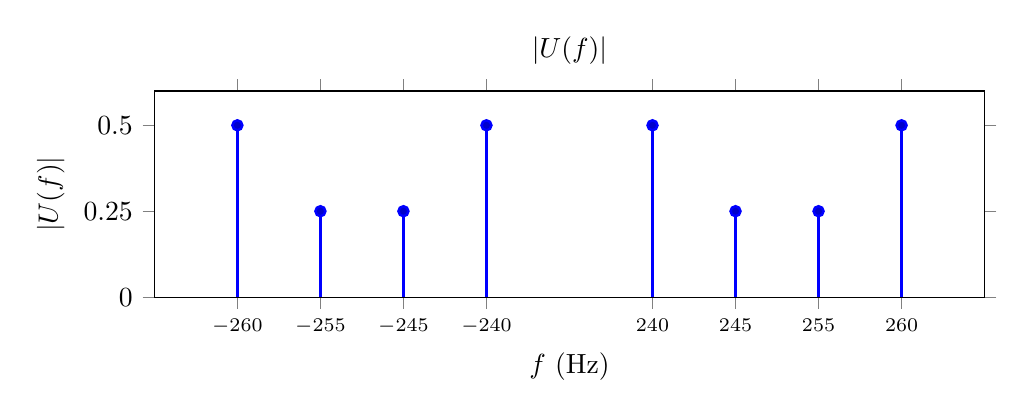
\begin{tikzpicture}
\begin{axis}[
    width=\linewidth,
    height=4.2cm,
    xlabel={$f$ (Hz)},
    ylabel={$|U(f)|$},
    xmin=-5, xmax=5,
    ymin=0, ymax=0.6,
    xtick={-4,-3,-2,-1,1,2,3,4},
    xticklabels={$-260$,$-255$,$-245$,$-240$,$240$,$245$,$255$,$260$},
    xticklabel style={font=\scriptsize},
    ytick={0,0.25,0.5},
    grid=none,
    tick align=outside,
    title={$|U(f)|$}
]
\addplot+[ycomb, mark=*, mark size=1.8pt, line width=0.9pt]
coordinates {(-4,0.5) (-3,0.25) (-2,0.25) (-1,0.5) (1,0.5) (2,0.25) (3,0.25) (4,0.5)};
\end{axis}
\end{tikzpicture}
\end{subfigure}
\hfill
\begin{subfigure}{0.32\linewidth}
\centering
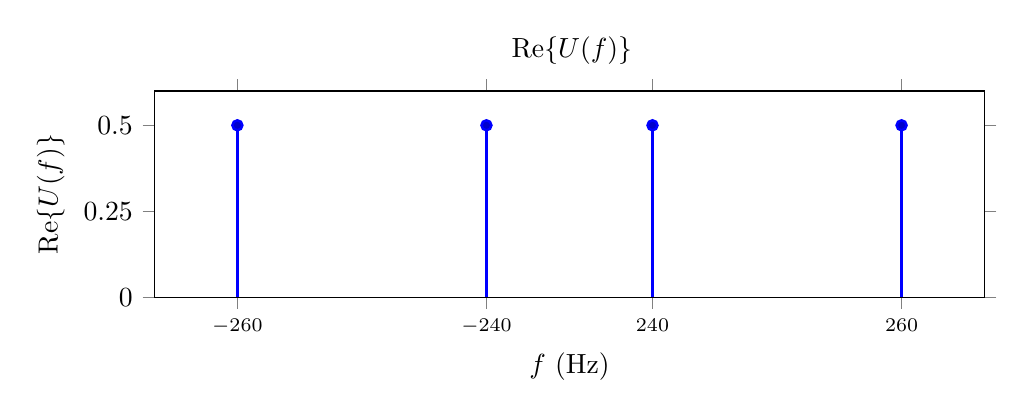
\begin{tikzpicture}
\begin{axis}[
    width=\linewidth,
    height=4.2cm,
    xlabel={$f$ (Hz)},
    ylabel={$\Re\{U(f)\}$},
    xmin=-5, xmax=5,
    ymin=0, ymax=0.6,
    xtick={-4,-1,1,4},
    xticklabels={$-260$,$-240$,$240$,$260$},
    xticklabel style={font=\scriptsize},
    ytick={0,0.25,0.5},
    grid=none,
    tick align=outside,
    title={$\,\Re\{U(f)\}$}
]
\addplot+[ycomb, mark=*, mark size=1.8pt, line width=0.9pt]
coordinates {(-4,0.5) (-1,0.5) (1,0.5) (4,0.5)};
\end{axis}
\end{tikzpicture}
\end{subfigure}
\hfill
\begin{subfigure}{0.32\linewidth}
\centering
\begin{tikzpicture}
\begin{axis}[
    width=\linewidth,
    height=4.2cm,
    xlabel={$f$ (Hz)},
    ylabel={$\Im\{U(f)\}$},
    xmin=-5, xmax=5,
    ymin=-0.3, ymax=0.3,
    xtick={-3,-2,2,3},
    xticklabels={$-255$,$-245$,$245$,$255$},
    xticklabel style={font=\scriptsize},
    ytick={-0.25,0,0.25},
    grid=none,
    tick align=outside,
    title={$\,\Im\{U(f)\}$}
]
\addplot+[ycomb, mark=*, mark size=1.8pt, line width=0.9pt]
coordinates {(-3,0.25) (-2,-0.25) (2,0.25) (3,-0.25)};
\end{axis}
\end{tikzpicture}
\end{subfigure}

\caption{Problem 3(b) sketches. Left: magnitude $|U(f)|$ with impulses at $\pm(240,245,255,260)\,\mathrm{Hz}$. Middle: real part (only at $\pm240,\pm260$) with weight $1/2$. Right: imaginary part (only at $\pm245,\pm255$) with weights $\pm 1/4$ arranged so $U(-f)=U^*(f)$.}
\end{figure}

\subsection*{(c) Lowpass filter for coherent demod}
The mixer output is
\[
y(t)=u(t)\cos(500\pi t)=m(t)\cos^2(500\pi t)=\frac{1}{2}\,m(t)\;+\;\frac{1}{2}\,m(t)\cos(1000\pi t).
\]
The baseband term is $\frac{1}{2}m(t)$ (support $\abs{f}\le \SI{10}{Hz}$); the second term sits around $\pm \SI{500}{Hz}$ (with $\pm 5$ and $\pm 10$\,Hz offsets). An \emph{ideal} LPF that passes baseband and rejects the high-frequency term, while restoring unity gain for $m(t)$, is:
\[
\boxed{\;
H(f)=
\begin{cases}
2, & |f|\le \SI{10}{Hz},\\
0, & |f|\ge \SI{240}{Hz},
\end{cases}
\quad\text{(any practical transition band between \SI{10}{Hz} and \SI{240}{Hz} is fine).}
\;}
\]
(The passband gain $2$ compensates the $\tfrac{1}{2}$ factor.)

\end{document}